%!TeX root = thesis-main.tex
\newcommand{\todos}[1]{\todo[inline, color=cyan]{\textbf{TODO}: #1}}
\newcommand{\constraints}[1]{\todo[inline, color=red]{#1}}
\newcommand{\suggestions}[1]{\todo[inline, color=yellow]{#1}}    
\newcommand{\hybridaggregate}[0]{AC+ML}


\sloppypar    
\chapter{Research Roadmap for Hybrid aggregate Computing}\label{chap:learning:roadmap}\mtcaddchapter
\minitoc % Creating an actual minitoc

Engineering of \ac{ac} applications 
 is a rich activity 
 that spans multiple concerns
 including
 designing the aggregate program,
 developing reusable algorithms~\cite{DBLP:conf/saso/AudritoCDV17,DBLP:journals/cee/AudritoCDPV21},  
 detailing the execution model~\cite{danilo2021lmcs},
 and choosing a deployment
 based on available infrastructure~\cite{DBLP:journals/fi/CasadeiPPVW20} (see \Cref{fig:architectures} for the full \ac{ac} ``stack'').
%
Traditionally,
 these activities have been carried out 
 through ad-hoc designs and implementations
 created by developers
 and tailored to specific contexts and goals (see Part II of the thesis),
 leading to, e.g.,
 self-organization algorithms 
 that are very reactive under certain network assumptions~\cite{DBLP:journals/cee/AudritoCDPV21},
 or round execution frequencies tailored to the velocity of change of underlying environment phenomena~\cite{danilo2021lmcs}.
%
To overcome the complexity and cost 
 of manually tailoring or devising general but inefficient algorithms, execution details, 
 and deployments,
 we propose to use \emph{\ac{ml} techniques}.
%
In particular, we observe that 
 automated design
 driven by learning
 can be applied at different levels
 of the \ac{ac} ``engineering stack''.
%
The integration of \ac{ac} and \ac{ml} done during this thesis, 
 which we refer to as \ac{acml} or \emph{hybrid} aggregate computing,
 is provided a lot of opportunities and challenges, 
 fostering a long-term record of research contributions.
%
In this chapter, we discuss a research roadmap followed during the thesis,
 for achieving the vision of hybrid aggregate computing.

\begin{figure}[h]
\centering
  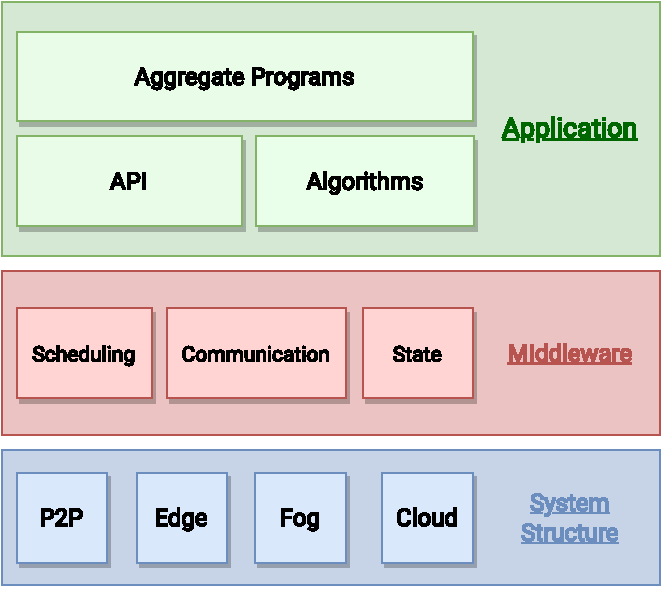
\includegraphics[width=0.8\linewidth]{papers/discoli/img/ac-rl.pdf}
  \caption[The aggregate computing stack]{The entire Aggregate Computing stack. 
  The application level (composed of API, algorithms and programs) needs to be supported by an execution platform/middleware, 
  to decouple the application from systems structures. 
  Then, this execution platform should be deployed in a particular architecture. 
  In our vision, \acl{ml} could enhance all of these layers.
  }
  \label{fig:architectures}
\end{figure}

\begin{figure}[h]
  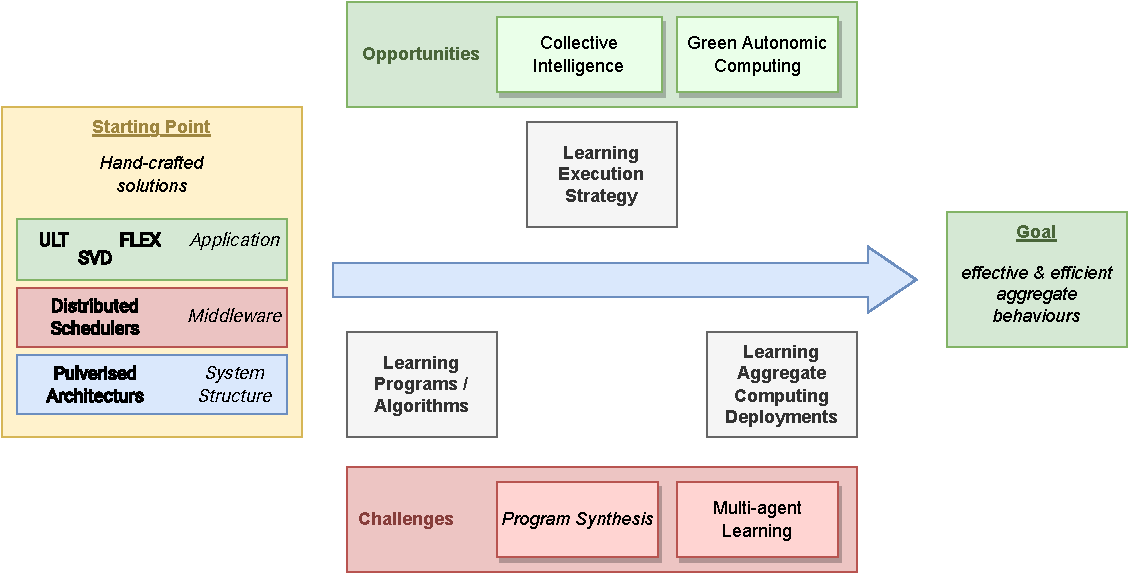
\includegraphics[width=\linewidth]{papers/discoli/img/roadmap.pdf}
  \caption[Overview of the research roadmap for combined aggregate computing with machine learning]{Overview of the research roadmap aiming at efficient and effective aggregate computations. 
  The starting point is current research, based on hand-crafted solutions.
  The goal is addressed through the application of hybrid aggregate computing at the program/execution/deployment levels.}
  \label{fig:roadmap}
\end{figure}

\section{Roadmap}\label{s:roadmap}

This section details motivation and direction for \ac{acml} research,
 also summarized in \Cref{fig:roadmap}.
%
%For a comprehensive introduction to \ac{ac},
% the reader can refer to~\cite{DBLP:journals/jlap/ViroliBDACP19}.

\subsection{Goals and Means}

To systematically analyse the 
 ways in which \ac{ml}
 can promote the development of 
 \ac{ac} applications, 
 it is important to 
 consider the \emph{goals} and \emph{means}
 of the \ac{ac} framework.
%

The goals include:
\begin{enumerate}
\item \emph{functionality} | achieving some collective behaviour (e.g., 
  environment monitoring and control through sensor-actuator networks~\cite{DBLP:journals/fi/CasadeiPPVW20,danilo2021lmcs},
 resiliently organize the system into leader-regulated areas~\cite{DBLP:conf/coordination/CasadeiPVN19},
 and 
 matching and coordinating collective tasks with worker ensembles~\cite{DBLP:journals/eaai/CasadeiVAPD21});

\item \emph{non-functionality} | concerning with the cost associated to the functionality.
\end{enumerate}
%
In particular, the latter can be further divided into multiple sub-goals from which application-specific \emph{trade-offs} can be made:
\begin{enumerate}
\item \emph{time efficiency}: refers to the time needed to converge to the desired state-of-affairs;
\item \emph{communication efficiency}: refers to the amount of communication performed (e.g., measured in terms of messages or bandwidth);
\item \emph{execution efficiency}: refers to the number of rounds of computations performed;
\item \emph{energy efficiency}: e.g. by combining communication and execution efficiency;
\item \emph{dependability}: concerns e.g. reliability or safety of a collective and its products. 
\end{enumerate}

In the \ac{ac} approach, 
 these goals can be addressed through three main means:
%
\begin{enumerate}
\item algorithms;
\item execution strategy;
\item system structure (deployment).
\end{enumerate}
%
Now, it turns out that \ac{ml}
 could be a powerful technique
 to replace
 or augment
 those traditionally human-engineered means.
\subsection{Patterns: learning \ac{ac} algorithms}

\ac{ac} algorithms 
 take collective inputs
 and use computational mechanisms
 to produce collective outputs.
%
In the \emph{field calculus}~\cite{DBLP:journals/jlap/ViroliBDACP19},
 the minimal formal framework 
 that underpins \ac{ac},
 collective inputs and outputs are denoted by
 \emph{computational fields} (or \emph{fields} for short), namely
 distributed data structures 
 mapping each device of the aggregate system to a value.
%
The field calculus, then, provides a set of operators
 for manipulating fields:
 essentially, operators specifying how fields evolve over time (round after round),
 and operators specifying interactions with neighbours
 (which can be reified through \emph{neighbouring fields}).
%
%
%The field calculus is implemented by so-called \emph{aggregate programming languages} such as \scafi{}, a Scala internal \ac{dsl}.
%
So, in \ac{ac}, a collective adaptive behaviour
 is the result of an algorithm (a function from fields to fields) expressed e.g. in \scafi{}
 and the concrete execution of the algorithm
 in a system of devices.
%

%A typical example is the \emph{gradient algorithm}~\cite{DBLP:conf/saso/AudritoCDV17},
 %which is essentially a function mapping a Boolean field of sources (i.e. the devices where the field is \emph{true})
 %to the field of minimum distances from those sources.
%
Usually, algorithms are \emph{progressive} -- they take time (computation rounds and communications) to converge to the ``correct'' value --
and \emph{self-healing}, i.e., they can adjust their output following changes in their inputs and the system topology.
%
For instance, a gradient algorithm progressively corrects the field of distances after the set of sources changes, or nodes move (hence changing the distances between neighbour nodes) or enter/leave the system.
%

So, different gradient algorithms may achieve the \emph{same} functionality (i.e., the eventual computation of the field of minimum distances from sources)
 with different non-functional outcomes.
%
Indeed, they may:
\begin{itemize}
  \item take a different time or a different number of rounds to converge, for the same initial condition;
  \item require a different amount of data to be exchanged;
  \item take different trade-offs e.g. regarding reactivity and smoothness (cf. the stability of values during change)~\cite{DBLP:journals/cee/AudritoCDPV21,DBLP:conf/saso/AudritoCDV17};
 or 
 \item take different assumptions regarding the execution model or the environment~\cite{DBLP:journals/cee/AudritoCDPV21}, which may affect applicability.
\end{itemize}
Designing efficient and versatile \ac{ac} algorithms can be complex~\cite{DBLP:journals/cee/AudritoCDPV21,DBLP:conf/saso/AudritoCDV17}: therefore, 
 it is interesting to explore
 whether algorithms can be learnt or synthesized
 given high-level functional goals.
%
For this purpose,
 an idea could be to combine
 the program synthesis~\cite{DBLP:journals/ftpl/GulwaniPS17} technique called \emph{sketching}~\cite{solar2008program-synthesis-sketching}
 with machine learning.
%
With this approach,
 the designer could provide an algorithm template
 with holes corresponding to actions
 to be learnt by the agents or the whole collective,
 e.g., through reinforcement learning.
%
In this case, learning would be used to \emph{search}
 for an optimal policy.
%
The resulting algorithm, then, would need extensive testing (e.g. by simulation) in a representative set of environments and dynamics.
%
In this regard, research is needed to identify what synthesis techniques, learning algorithms, frameworks, and methodologies can support the learning of algorithms able to achieve performance similar or better than state-of-the-art solutions.
%
The first effort in this direction has been done in~\cite{DBLP:conf/coordination/CasadeiPVN19}, where a gradient algorithm has been learnt through a reinforcement learning approach~\Cref{chap:learning:sketching}.

\subsection{Platform: learning execution strategies and adaptations}

For a given \ac{ac} program or algorithm,
  multiple execution strategies can be applied,
  affecting aspects like
  the scheduling of computation rounds (i.e., the frequency of execution),
  the scheduling of communications (i.e., when the devices exchange data),
  the retention of messages from neighbours (i.e., when should messages from the neighbour be considered too old to be used).
%
In particular,
 a first distinction 
 can be made between \emph{static}
 and \emph{dynamic} execution strategies.
%
The latter approaches adapt the execution choices
 at runtime depending on factors
 which may include
 the speed of environmental change,
 the energy level of a device,
 incentives in volunteering settings,
 or the desired \ac{qos}.
%
Moreover, these factors may be diverse 
 in diverse portions of the system;
 so, it is in general important to also consider
 the local context of each device or set of devices.

Note that adaptive behaviour
 could be achieved via static execution strategies, e.g., by using reactive approaches triggering behaviours when specific context conditions apply~\cite{danilo2021lmcs}.
%
However, again, 
 since it is in general hard to design static or dynamic execution strategies 
 able to adequately take into account all the factors and goals,
 it could make sense to let a system (and its components) learn 
 how to efficiently execute algorithms 
 according to a set of given high-level objectives.
%
Indeed, true adaptiveness 
 comes from changing the behavioural rules,
 and learning is a premier tool for 
 changing for the better.
%
The emphasis on improving efficiency
 by optimizing execution 
 of aggregate systems,
 hence promoting sustainability
 of collective computations,
 could be the opportunity to open up a vision 
 of \emph{green autonomic computing}.
%
In~\cite{aguzzi2022coord-ac-rl} the authors have proposed a reinforcement learning approach to learn the execution strategy to improve the execution efficiency of a gradient algorithm. %TODO add reference to the right chapter.
\subsection{Platform: learning system structures and re-structuring}
A logical \ac{ac} system 
 consists of a logical network
 of logical devices
 operating as per the aforementioned execution protocol.
%
It is the \emph{collective digital twin}~\cite{casadei2022applsci}
 of a target set of application-level physical devices (e.g., robots of a swarm, or workers in a computing ecosystem).
%
As shown in recent work on \emph{pulverized architectures}~\cite{DBLP:journals/fi/CasadeiPPVW20},
 it turns out that different application partitioning schemas and implementations of the \emph{digital thread} associated with the aggregate system are possible,
 as well as different deployments
 of application components
 onto the available \ac{ict} infrastructure.
%
%
For instance,
 it is possible to embed evaluations of the aggregate program into the devices themselves,
 to move the entire computational part to the cloud (leaving devices as thin hosts dealing only with sensing and actuation),
 or spread these onto a layer of edge-fog infrastructural devices.
%
Different deployments 
 may lead to different efficiency trade-offs
 and non-functional outcomes~\cite{DBLP:journals/fi/CasadeiPPVW20,casadei2022applsci},
 which, crucially, may also change dynamically 
 due to application and infrastructure dynamics
 (cf. addition or removal of new nodes, blackouts, etc.).
 

In previous research, aggregate application partitioning and deployment have been done manually at design time~\cite{DBLP:journals/fi/CasadeiPPVW20}---as showed in \Cref{chap:eng:multitier}.
%
However, for a given set of infrastructures, it is not easy to determine an \emph{effective} mapping.
%
The usual approach consists of manually generating different deployments,
 simulating these for the same set of applications,
 collecting various cost metrics,
 and evaluating results to determine trade-offs and guidelines.
%
However, \ac{ml} could be \emph{injected} into 
 such a methodology
 to have the system learn by itself what is a
 (locally) optimal deployment for an aggregate application.
% 
Moreover, the system could be induced to learn a strategy to self-adapt the deployment (i.e., by moving components opportunistically across the \ac{ict} infrastructure) 
 while trying to preserve, e.g., certain \ac{qos} targets.
 
Additionally,
 it has been shown in \cite{casadei2022applsci},
 that changing the logical structure of an aggregate system at runtime
 (e.g., by injecting \emph{virtual} devices)
 could be a further means 
 for steering self-organization processes,
 namely to improve the collective behaviour of a system (cf. \cite{DBLP:journals/jnca/LiS11}).
%
In this respect,
 a challenge would be to determine
 \emph{how}, \emph{when}, and \emph{where} 
 virtual devices
 should be spawned or removed
 from the system.
%
In the \ac{acml} vision,
 this problem should not be addressed
 through ad-hoc solutions,
 but the \ac{ac} system should be trained
 in order to learn the best strategies
 for improving the efficacy and efficiency
 of aggregate applications.
\section{Opportunities and Challenges}

%The research delineated in \Cref{s:roadmap}
% is rich in opportunities and challenges---the most significant ones discussed in the following.

\subsection*{Opportunities}

A prominent opportunity of \ac{acml} research lies 
 in potentially getting insights 
 about the \emph{automatic design 
 of \acf{ci}},
 renewing the partial contributions
 given by Szuba's computational collective intelligence~\cite{DBLP:journals/fgcs/Szuba01}
 and Tumer and Wolpert's COIN (COllective INtelligence)~\cite{DBLP:journals/jair/WolpertT02}.
%
However, unlike previous work, 
 the peculiar characteristic of aggregate computing 
 of reifying \ac{ci} into macro-level \emph{programs}
 (which we may refer to as \emph{\ac{ci} programmability})
 is expected to enable a synergic and gentle introduction of automatic design and learning.
%
Additionally, the other crucial aspect of
 functional \emph{compositionality} of aggregate behaviours (denoted by functions operating on fields),
 is also expected to help, e.g.,
 by fostering learning processes
 whereby the goal is to find suitable compositions of elementary collective behaviours.
%
Moreover, the ability to change execution strategies while guaranteeing the same behaviour could also be considered a form of \ac{ci}.

Indeed, another key opportunity 
 lies in the possibility of fostering \emph{efficiency}
 in large-scale intelligent systems,
 which is more and more important
 for sustainability
 as advocated by important fields
 like \emph{green computing}~\cite{DBLP:journals/iet-net/SarkarM16}.
%
The significance of the problem 
 is especially relevant nowadays because
 of the tension between
 the visions of pervasive computing~\cite{DBLP:journals/computer/SahaM03}, future-generation large-scale computational collectives~\cite{DBLP:journals/eaai/CasadeiVAPD21}, and autonomic computing (promoting smarter -- i.e. more computationally intensive -- devices)~\cite{DBLP:journals/computer/KephartC03}
 and the urge to limit the impact
 of humans and technologies on the environment.
%
\subsection*{Technical Challenges}

Applying learning through the \ac{ac} stack (\Cref{fig:architectures}) poses several challenges,
 many of which are implied by 
 the nature of aggregate systems---cf.
 distribution, 
 decentralization, 
 partial observability,
 many-agents coordination, and
 the eventual nature of collective computations,
  
%due to the peculiarities which those systems manifest, mainly associated with the multi-agent cooperative settings and \emph{partial environment} observability.

Particularly, learning in \emph{many}-agent networked system~\cite{DBLP:journals/jzusc/ZhangYB21} is currently an open challenge.
%
Indeed, extending the learning from one agent to many agents exponentially enlarges the policy search space, due to the combinatorial nature of multi-agent systems~\cite{DBLP:journals/aamas/Hernandez-LealK19}.
%
Moreover, the neighbouring-based system structure is not strict and could evolve in time, leading to time- and space-varying input spaces.
%
Furthermore, it is not appropriate to use a centralized controller that orchestrates the system as a whole, due to the typical large scale and resilience requirements.
%
However, using only a local vision of the system could lead to the problem of \emph{non-stationarity}, since each agent concurrently learns and modifies the environment in the eye of the other agents~\cite{DBLP:journals/aim/TuylsW12}.
%
Another concern related to many-agent settings is the \emph{multi-agent credit assignment} problem~\cite{sutton-book}.
%
This is referred to in the difficulty of deriving a local reward policy from a global utility that measures the system as a whole~\cite{DBLP:conf/atal/AgoginoT04}. 
%
Besides, the reward received is typically very delayed and sparse in time, because an action taken in a point of large geographical space, could lead to an influence on the whole system only when it reaches all nodes.

These challenges are mitigated 
 by an increasing track of research records on \ac{ac}~\cite{DBLP:journals/jlap/ViroliBDACP19},
 the availability of formal tools for 
 analysing and reasoning about aggregate computations and systems~\cite{DBLP:journals/jlap/ViroliBDACP19},
 and the support given by tools for 
 developing and simulating aggregate systems~\cite{DBLP:journals/jlap/ViroliBDACP19}.
\section{Final Remarks}
%
Developing \ac{ac} applications
 requires addressing
 various
 algorithmic,
 computational,
 and deployment concerns.
%
The integration of \ac{ml} 
 across the \ac{ac} development stack
 provides opportunities and challenges
 requiring significant research.
%
The roadmap for \ac{acml} delineated in this thesis
 is expected to provide results and insights
 on the engineering of collectively intelligent distributed systems.
%
In the ensuing chapters, we will elaborate on the efforts delineated by this roadmap, 
 which align with the facets defined during the engineering phase. 
 Specifically concerning high-level aspects (i.e., the design patterns), 
 we first introduce an approach called ``Collective Program Sketching''~\Cref{chap:learning:roadmap}.
 This method enables the definition of partial collective algorithms with intentional gaps, 
 subsequently filled via machine learning techniques. 
 Additionally, 
 we introduce a distinct yet related concept called ``Field-informed reinforcement learning''~\Cref{chap:rl:field-informed} .
 In this context, aggregate computing is employed to enhance the collective learning process. 
 The computational fields generated by aggregate computing serve 
 to inform the learning process with collective knowledge, 
 despite the existence of only local knowledge.

Subsequently, we shifted our focus to platform facets. 
 The initial endeavour in this realm culminated in the development of ``distributed schedulers''~\cref{chap:rl:schedulers}, 
 wherein RL has been utilized to augment the efficiency of a self-stabilizing collective computation. 
 The experience gained from these three projects has led to the creation of a specialized tool named ``ScaRLib''~\Cref{chap:rl:scarlib}. 
 This tool serves as an enabling medium towards a hybrid vision of aggregate computing and is particularly well-suited for supporting many-agent learning vision.
%\printbibliography
